\documentclass[]{article}
%Busca la linea que pone /tableofcontents y empieza a escribir debajo de cada sección.
%Te explico para qué es cada cosa que sea medio relevante:
\usepackage{amsmath}
\usepackage{amssymb}
\usepackage{verbatim} %con verbatim escribes bloques de texto con letra mono.
\usepackage{graphicx} %para insertar imagenes, cuando meta yo una usa el codigo de ejemplo
\usepackage{listings}
\usepackage{fullpage}
\usepackage{color}
\usepackage{fancyvrb}
\usepackage[spanish]{babel}
\usepackage[utf8]{inputenc} %Para usar acentos directamente en latex
\usepackage{hyperref} %Para que el indice tenga hiperenlaces y si quieres poner los tuyos
\hypersetup{%
	pdfborder = {0 0 0}
}

\definecolor{mygreen}{rgb}{0,0.6,0}
\definecolor{mygray}{rgb}{0.5,0.5,0.5}
\definecolor{mymauve}{rgb}{0.58,0,0.82}

%Para insertar código: crea un recuadro con texto mono y lineas enumeradas. Puedes referenciar un fichero y no copiar y pegar aquí.
\lstset{ %
	backgroundcolor=\color{white},   % chohttp://xdxd.com/ose the background color; you must add \usepackage{color} or \usepackage{xcolor}
	basicstyle=\footnotesize,        % the size of the fonts that are used for the code
	breakatwhitespace=false,         % sets if automatic breaks should only happen at whitespace
	breaklines=true,                 % sets automatic line breaking
	captionpos=b,                    % sets the caption-position to bottom
	commentstyle=\color{mygreen},    % comment style
	frame=single,                    % adds a frame around the code
	keepspaces=true,                 % keeps spaces in text, useful for keeping indentation of code (possibly needs columns=flexible)
	numbers=left,                    % where to put the line-numbers; possible values are (none, left, right)
	numbersep=5pt,                   % how far the line-numbers are from the code
	numberstyle=\tiny\color{mygray}, % the style that is used for the line-numbers
	rulecolor=\color{black},         % if not set, the frame-color may be changed on line-breaks within not-black text (e.g. comments (green here))
	showspaces=false,                % show spaces everywhere adding particular underscores; it overrides 'showstringspaces'
	showstringspaces=false,          % underline spaces within strings only
	showtabs=false,                  % show tabs within strings adding particular underscores
	stepnumber=1,                    % the step between two line-numbers. If it's 1, each line will be numbered
	stringstyle=\color{mymauve},     % string literal style
	tabsize=4,
	inputencoding=utf8,
	title=\lstname                   % show the filename of files included with \lstinputlisting; also try caption instead of title
}



\title{Servicios Telemáticos Avanzados}
\author{José Luis Cánovas Sánchez\\Ezequiel Santamaría Navarro}

\begin{document}

\maketitle

\begin{abstract}
%Aquí el resumen
\end{abstract}

\tableofcontents


\section{Introducción}

Somos el grupo 3, así que nos encargaremos de las organizaciones 31 y 32.

\section{Topología}

En esta sección describimos la forma en la que se van a desplegar los servicios y como estarán
conectados entre sí.

\subsection{Dispositivos}

Tenemos para las pruebas y el desarrollo de la práctica, las siguientes herramientas hardware:

\begin{itemize}

	\item Un \textbf{switch} con VLAN y 5 puertos.
	\item Un ordenador que actúa de \textbf{enrutador}, con dos puertos ethernet, uno de ellos con configuración VLAN.
	\item Un \textbf{punto de acceso} WiFi para el acceso a la red.
	\item Un \textbf{iPhone} y un \textbf{portátil Mac}, útiles para probar VOIP con wifi.
	\item Dos ordenadores que actúan como \textbf{organizaciones} 31 y 32.
	\item Dos ordenadores más para simular \textbf{clientes} haciendo peticiones.

\end{itemize}

\subsection{Topología de red}

%TODO: explicar la topología lógica: un server, 1-2 clientes, a lo sumo un server extra.

En cuanto a la topología física real, disponemos en el laboratorio de 3 torres, 5 puertos del switch CISCO y un punto de acceso wifi configurado para la organización 31. La conexión del una de las torres como router y las otras dos como equipos de cada organización ya se explica en los boletines de prácticas.
\\

A partir de esa configuración básica, configuramos las dos organizaciones de manera casi simétrica: en la máquina física de una organización, se ejecutarán como máquinas virtuales un servidor y uno o dos clientes para probar los servicios. Decidimos usar un servidor porque la cantidad de servicios proporcionados por una organización no son tan pesados como carga de trabajo para una única máquina, como lo pueda ser tener varios servidores como máquinas virtuales en la misma torre del laboratorio. En la organización 32 podrían haber dos servidores para, por ejemplo, probar la gestión de servidor con SNMP que no sean en la misma máquina.
\\

Ahora bien, por el modo en que programamos la configuración de dispositivos, nos es muy fácil cambiar los roles de las máquinas de modo que el servidor de una organización sea la máquina física, y los clientes una máquina virtual, o una torre libre del laboratorio, o un móvil o portátil nuestros.
\\

Con esto nuestra solución para la práctica se centra más en los dispositivos lógicos \textit{SERVER}, \textit{CLIENTE}, \textit{ROUTER}, que en las máquinas que disponemos en los laboratorios o las máquinas virtuales creadas.


\begin{figure}[h!]
	\caption{Topología física}
	\centering
		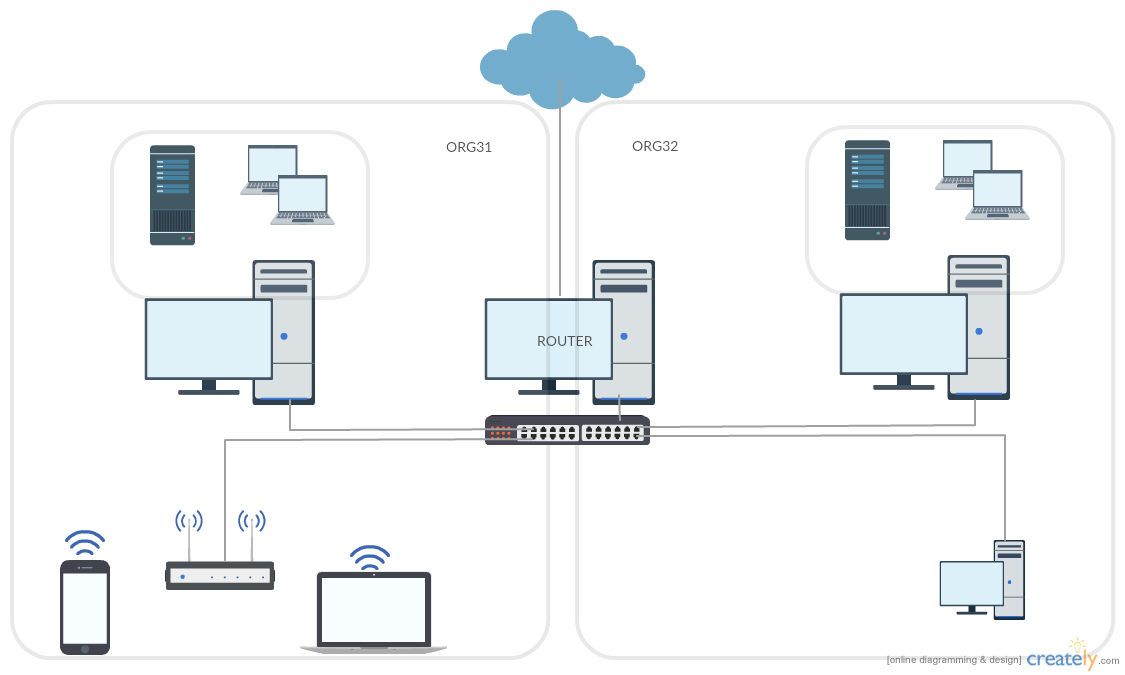
\includegraphics[scale=0.35]{images/TopologiaFisica}
\end{figure}

\section{Configuración de los dispositivos}

Para la configuración de los dispositivos utilizamos herramientas Makefile, y scripts escritos en bash y python, de manera que desplegar los servicios y la topología en un dispositivo esté automatizado. No nos apoyamos en una máquina virtual que vayamos configurando a lo largo de las prácticas llevándola de un lado a otro, y por lo general, usamos máquinas virtuales con una instantánea \textit{limpia}.
\\

Usamos una estructura de directorios basada en el hardware a configurar. Es decir, en el ordenador que hace de enrutador ejecutamos un Makefile que está en el directorio ROUTER.

%TODO: decidir si se pone la estructura, y si se modifica cómo presentarla.
\begin{Verbatim}
ROUTER
	SNMP
	Makefile
	network
	test
ORG1
	FISICA
		Makefile
		network
		test
	SERVER
		SNMP
		VOIP
		Makefile
		network
		test
	CLIENTE1
		SNMP
		VOIP
		Makefile
		network
		test

\end{Verbatim}

\section{Servicios}

\subsection{Enrutamiento}

Del enrutamiento se encarga el PC que hace de enrutador. La configuración física se basa en tres puertos Ethernet:

\begin{itemize}
	\item Un puerto se usa para conectarse a la red de la UMu, que da conectividad al exterior.
	\item Otro puerto, conectado al \textit{trunk switch vlan} de la organización 31.
	\item Ídem, para la organización 32.
\end{itemize}

La configuración lógica, es decir, la configuración de los interfaces de red es la siguiente:

\begin{lstlisting}
TODO: Copiar la configuracion de las interfaces.
\end{lstlisting}
\lstinputlisting{../ROUTER/network}

\subsection{SNMP}

\subsubsection{Agentes}

\subsubsection{Manejador}

\subsection{Voz sobre IP}

En esta sección documentamos las configuraciones que hemos tomado para el servidor de Asterisk.

\subsubsection{Configuración básica}

Para las organizaciones 31 y 32, hacemos 2 cuentas de cliente para ambas organizaciones (311 y 312 para organización 31; 321 y 322 para la organización 32).

\begin{lstlisting}
TODO: Copiar aqui la configuracion relativa a los clientes.
\end{lstlisting}

Para esos clientes también hemos configurado sus extensiones.

\begin{lstlisting}
TODO: Copiar aqui la configuracion relativa a las extensiones.
\end{lstlisting}

\subsubsection{Troncales Asterisk}

Para empezar, hacemos una redirección básica entre los dos servicios Asterisk en las configuraciones de extensión de Asterisk:

\begin{lstlisting}
TODO: Copiar aqui la configuracion relativa a las extensiones entre servicios.
\end{lstlisting}

\subsubsection{Buzón de voz}

\subsection{LDAP}
El servicio LDAP ofrece al resto de servicios un punto en común donde encontrar la información relevante de los usuarios (nombres,
organización a la que pertenecen, permisos de uso y acceso, credenciales, etc).

Como contiene la información crítica de los usuarios que se integran en los servicios, LDAP se despliega en su propia máquina.

Sin embargo, en el despliegue real del laboratorio, LDAP está integrado en el ordenador de la organización 31.

Para las pruebas de laboratorio, la instalación y la configuración la generamos automáticamente (sin necesidad de
interacción del administrador), en python, generando tres clientes de la organización 31.

%TODO: Incluir partes o total del fichero python.
%TODO: Incluir un ldiff y comentarlo.
%TODO: Describir qué es db.tar.gz e initial.tar.gz
%TODO: Justificar que funciona correctamente con ldapsearch.
%TODO: LDAP lo integramos con OwnCloud y lo probamos.

\subsection{OwnCloud}

\section{Políticas de seguridad}
%TODO: Un dibujo del escenario de seguridad

\subsection{Análisis de riesgos}
%TODO: Tabla de reglas de seguridad

\subsection{Configuración de seguridad}
%TODO: Iptables

\subsection{Generación de certificados}
En openssl.cnf no se explica que %yo me entiendo

[ usr_cert ]

crlDistributionPoints = URI:http://server.org31/crl/org31.CRL

\end{document}
